\documentclass[aspectratio=169,11pt]{beamer}

\usetheme{Madrid}
\usecolortheme{seahorse}
\usefonttheme{professionalfonts}

\usepackage[T1]{fontenc}
\usepackage[utf8]{inputenc}
\usepackage{amsmath,amssymb}
\usepackage{booktabs}
\usepackage{tikz}
\usetikzlibrary{arrows.meta,positioning,shapes.geometric}

\definecolor{LaxTeal}{HTML}{087F8C}
\definecolor{LaxGreen}{HTML}{3D7D4F}
\definecolor{LaxAmber}{HTML}{C27B29}
\definecolor{LaxRed}{HTML}{B24F4B}
\definecolor{LaxInk}{HTML}{202521}
\definecolor{LaxMuted}{HTML}{667067}
\definecolor{LaxPaper}{HTML}{F4F6F2}

\setbeamercolor{palette primary}{bg=LaxTeal,fg=white}
\setbeamercolor{palette secondary}{bg=LaxGreen,fg=white}
\setbeamercolor{palette tertiary}{bg=LaxAmber,fg=white}
\setbeamercolor{frametitle}{bg=LaxTeal,fg=white}
\setbeamercolor{title}{fg=LaxInk}
\setbeamercolor{block title}{bg=LaxTeal,fg=white}
\setbeamercolor{block body}{bg=LaxPaper,fg=LaxInk}
\setbeamercolor{alerted text}{fg=LaxRed}
\setbeamertemplate{navigation symbols}{}
\setbeamertemplate{itemize item}{\color{LaxTeal}$\blacktriangleright$}
\setbeamertemplate{itemize subitem}{\color{LaxAmber}$\circ$}

\newcommand{\EvidenceRule}{\textbf{Evidence first. Claims later.}}
\newcommand{\ZCR}{\ensuremath{U_t - V_x + [U,V] = 0}}
\newcommand{\Pipeline}{generate $\rightarrow$ solve $\rightarrow$ reduce $\rightarrow$ falsify $\rightarrow$ extract structure $\rightarrow$ review}

\title[LAXFORGE + LAXCERT]{LAXFORGE and LAXCERT}
\subtitle{Gauge-aware evidence for Lax-pair discovery}
\author{LAXFORGE Project}
\date{Extended poster-style presentation}

\begin{document}

\begin{frame}[plain]
  \titlepage
  \vspace{-0.6cm}
  \begin{center}
    \Large \EvidenceRule
  \end{center}
\end{frame}

\begin{frame}{Poster Snapshot}
  \begin{columns}[T,totalwidth=\textwidth]
    \begin{column}{0.32\textwidth}
      \begin{block}{What LAXFORGE Is}
        A gauge-aware discovery and audit engine for zero-curvature
        representations, Lax pairs, and integrable-systems candidates.
      \end{block}
      \begin{block}{What It Produces}
        Candidate dossiers: formulas, curvature evidence, gauge-risk notes,
        invariant fingerprints, structure attempts, and prior-art collision
        records.
      \end{block}
    \end{column}
    \begin{column}{0.32\textwidth}
      \begin{block}{What LAXCERT Adds}
        A certificate-validation boundary for compatible LAXFORGE exports.
        LAXFORGE proposes structured artifacts; LAXCERT checks the certificate
        side.
      \end{block}
      \begin{block}{What It Does Not Do}
        It does not prove novelty, guarantee integrability, or automate
        publication. Novelty remains a human-reviewed mathematical conclusion.
      \end{block}
    \end{column}
    \begin{column}{0.32\textwidth}
      \begin{block}{Core Equation}
        \[
          \ZCR
        \]
        The zero-curvature condition asks whether two symbolic directions are
        compatible without residual obstruction.
      \end{block}
      \begin{block}{Operating Standard}
        \centering
        \Pipeline
      \end{block}
    \end{column}
  \end{columns}
\end{frame}

\begin{frame}{Lay Background: Why This Exists}
  \begin{columns}[T,totalwidth=\textwidth]
    \begin{column}{0.48\textwidth}
      \begin{block}{The Research Problem}
        Many equations in physics and geometry are nonlinear: small effects can
        interact in complicated ways. Integrable systems are special because
        they carry hidden structure that can make them unusually tractable.
      \end{block}
      \begin{block}{A Lax Pair, Plainly}
        A Lax pair is a pair of mathematical instructions that watch the same
        motion from two directions. If the instructions agree perfectly, their
        agreement can encode the equation being studied.
      \end{block}
    \end{column}
    \begin{column}{0.48\textwidth}
      \begin{alertblock}{Why Caution Is Needed}
        A symbolic search can produce formulas that look impressive while
        hiding familiar, fake, reducible, or parameter-removable structure.
      \end{alertblock}
      \begin{block}{LAXFORGE's Role}
        LAXFORGE turns a raw symbolic hit into an evidence trail. The candidate
        is not the conclusion; it is the object under test.
      \end{block}
    \end{column}
  \end{columns}
\end{frame}

\begin{frame}{The Metal-Detector Analogy}
  \begin{columns}[T,totalwidth=\textwidth]
    \begin{column}{0.40\textwidth}
      \begin{block}{A Raw Search Hit}
        A symbolic search result is like a detector beep. It indicates that
        something may be present, but it does not identify, value, or validate
        the object.
      \end{block}
      \begin{block}{The Follow-Up Work}
        LAXFORGE performs the mathematical equivalent of digging, cleaning,
        testing, comparing, labeling, and deciding whether an expert should
        inspect the result.
      \end{block}
    \end{column}
    \begin{column}{0.56\textwidth}
      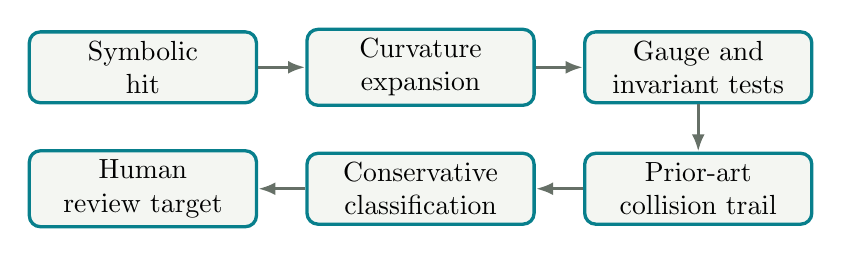
\begin{tikzpicture}[
        node distance=0.6cm,
        box/.style={rectangle,rounded corners,draw=LaxTeal,very thick,align=center,
          fill=LaxPaper,minimum height=0.9cm,text width=2.65cm},
        arrow/.style={-{Latex[length=2.2mm]},very thick,draw=LaxMuted}
      ]
        \node[box] (beep) {Symbolic\\hit};
        \node[box,right=of beep] (dig) {Curvature\\expansion};
        \node[box,right=of dig] (test) {Gauge and\\invariant tests};
        \node[box,below=of test] (compare) {Prior-art\\collision trail};
        \node[box,left=of compare] (label) {Conservative\\classification};
        \node[box,left=of label] (review) {Human\\review target};
        \draw[arrow] (beep) -- (dig);
        \draw[arrow] (dig) -- (test);
        \draw[arrow] (test) -- (compare);
        \draw[arrow] (compare) -- (label);
        \draw[arrow] (label) -- (review);
      \end{tikzpicture}
    \end{column}
  \end{columns}
\end{frame}

\begin{frame}{What Goes Into LAXFORGE}
  \begin{columns}[T,totalwidth=\textwidth]
    \begin{column}{0.31\textwidth}
      \begin{block}{Fields and Variables}
        Unknown functions such as $u$, $v$, $p$, or $q$, usually depending on
        space $x$ and time $t$.
      \end{block}
    \end{column}
    \begin{column}{0.31\textwidth}
      \begin{block}{Coefficient Algebra}
        The symbolic setting in which coefficients live: scalar expressions,
        truncated polynomial algebras, finite algebras, or other structured
        systems.
      \end{block}
    \end{column}
    \begin{column}{0.31\textwidth}
      \begin{block}{Ansatz and Constraints}
        A structured guess for $U$ and $V$, plus degree limits, symmetry
        assumptions, target equations, or search-lane restrictions.
      \end{block}
    \end{column}
  \end{columns}
  \vspace{0.35cm}
  \begin{block}{Why an Ansatz Matters}
    The universe of formulas is too large to search blindly. A good ansatz is a
    well-designed experiment: narrow enough to check, broad enough to reveal
    useful structure.
  \end{block}
\end{frame}

\begin{frame}{Core Workflow}
  \begin{tikzpicture}[
    node distance=0.5cm,
    step/.style={rectangle,rounded corners,draw=LaxTeal,thick,fill=LaxPaper,
      align=center,text width=2.4cm,minimum height=0.85cm},
    gate/.style={diamond,aspect=2.2,draw=LaxAmber,thick,fill=white,
      align=center,text width=2.0cm},
    arrow/.style={-{Latex[length=2mm]},thick,draw=LaxMuted}
  ]
    \node[step] (arena) {Arena and ansatz};
    \node[step,right=of arena] (solve) {Generate and solve};
    \node[gate,right=of solve] (curv) {Curvature zero?};
    \node[step,right=of curv] (reduce) {Gauge reduction};
    \node[step,below=of reduce] (fp) {Fingerprints and structure};
    \node[step,left=of fp] (prior) {Prior-art check};
    \node[gate,left=of prior] (classify) {Review worthy?};
    \node[step,left=of classify] (dossier) {Emit dossier};
    \draw[arrow] (arena) -- (solve);
    \draw[arrow] (solve) -- (curv);
    \draw[arrow] (curv) -- node[above]{yes} (reduce);
    \draw[arrow] (curv) -- ++(0,-1.2) -| node[pos=0.25,left]{no: record residuals} (dossier);
    \draw[arrow] (reduce) -- (fp);
    \draw[arrow] (fp) -- (prior);
    \draw[arrow] (prior) -- (classify);
    \draw[arrow] (classify) -- (dossier);
  \end{tikzpicture}
  \vspace{0.2cm}
  \begin{center}
    \small Every branch should leave evidence: pass, fail, warning, or blocked.
  \end{center}
\end{frame}

\begin{frame}{Zero Curvature and Coefficient Splitting}
  \begin{columns}[T,totalwidth=\textwidth]
    \begin{column}{0.46\textwidth}
      \begin{block}{The Calculation}
        \[
          \ZCR
        \]
        LAXFORGE expands this expression over the relevant matrix entries,
        algebra basis elements, derivatives, and spectral-parameter powers.
      \end{block}
      \begin{block}{If It Cancels}
        The pair may encode a PDE or a target flow. The dossier records the
        proof structure rather than relying on a visual simplification.
      \end{block}
    \end{column}
    \begin{column}{0.50\textwidth}
      \begin{alertblock}{If It Does Not Cancel}
        The residual is still useful. It records what failed, which basis terms
        remained, and whether the search lane should be discarded or refined.
      \end{alertblock}
      \begin{block}{Coefficient Splitting}
        A single symbolic expression can hide many independent checks.
        Splitting turns ``looks zero'' into a list of explicit obligations.
      \end{block}
    \end{column}
  \end{columns}
\end{frame}

\begin{frame}{Gauge Risk: Same Structure, Different Costume}
  \begin{columns}[T,totalwidth=\textwidth]
    \begin{column}{0.50\textwidth}
      \begin{block}{Plain-Language Meaning}
        A gauge transformation is a change of mathematical description. Two
        formulas may look different while representing the same underlying
        structure.
      \end{block}
      \begin{block}{Why It Matters}
        Without gauge checks, a search engine can overcount old mathematics,
        preserve fake pairs, or mistake removable parameters for meaningful
        spectral information.
      \end{block}
    \end{column}
    \begin{column}{0.46\textwidth}
      \begin{block}{Evidence LAXFORGE Tracks}
        \begin{itemize}
          \item parameter-removal tests;
          \item block-reducibility checks;
          \item cyclic-basis or invariant fingerprints;
          \item known projection and collision notes;
          \item explicit unsupported or blocked states.
        \end{itemize}
      \end{block}
    \end{column}
  \end{columns}
\end{frame}

\begin{frame}{Candidate Dossier: Poster Checklist}
  \begin{columns}[T,totalwidth=\textwidth]
    \begin{column}{0.33\textwidth}
      \begin{block}{Definition}
        \begin{itemize}
          \item fields and variables;
          \item coefficient algebra;
          \item candidate pair $(U,V)$;
          \item generated or target PDE.
        \end{itemize}
      \end{block}
      \begin{block}{Curvature}
        \begin{itemize}
          \item full expansion;
          \item coefficient basis;
          \item residual-zero flag;
          \item unresolved terms.
        \end{itemize}
      \end{block}
    \end{column}
    \begin{column}{0.33\textwidth}
      \begin{block}{Reduction}
        \begin{itemize}
          \item gauge-risk report;
          \item fake-pair assessment;
          \item spectral-parameter status;
          \item reducibility notes.
        \end{itemize}
      \end{block}
      \begin{block}{Structure}
        \begin{itemize}
          \item invariant fingerprints;
          \item conservation-law attempts;
          \item Hamiltonian attempts;
          \item recursion or hierarchy evidence.
        \end{itemize}
      \end{block}
    \end{column}
    \begin{column}{0.28\textwidth}
      \begin{block}{Review}
        \begin{itemize}
          \item known-family collisions;
          \item failure reasons;
          \item gate summary;
          \item conservative classification.
        \end{itemize}
      \end{block}
      \begin{alertblock}{Key Rule}
        A candidate dossier can become a human review target. It is not a
        novelty claim.
      \end{alertblock}
    \end{column}
  \end{columns}
\end{frame}

\begin{frame}{LAXCERT: The Certificate Boundary}
  \begin{columns}[T,totalwidth=\textwidth]
    \begin{column}{0.48\textwidth}
      \begin{block}{LAXFORGE Side}
        \begin{itemize}
          \item proposes structured candidate artifacts;
          \item emits provenance and source reports;
          \item records assumptions and trust boundaries;
          \item keeps discovery separate from certification.
        \end{itemize}
      \end{block}
      \begin{block}{Example Export}
        \texttt{candidate.json}\\
        \texttt{laxforge\_manifest.json}\\
        \texttt{source\_report.json}
      \end{block}
    \end{column}
    \begin{column}{0.48\textwidth}
      \begin{block}{LAXCERT Side}
        \begin{itemize}
          \item consumes compatible artifacts;
          \item validates against its schema;
          \item checks the certificate strategy;
          \item reports validation status independently.
        \end{itemize}
      \end{block}
      \begin{alertblock}{Clean Claim}
        LAXFORGE prepares and documents the sample. LAXCERT checks the
        certificate. Expert judgment remains outside the automation boundary.
      \end{alertblock}
    \end{column}
  \end{columns}
\end{frame}

\begin{frame}{Calibration, Not Novelty}
  \begin{columns}[T,totalwidth=\textwidth]
    \begin{column}{0.50\textwidth}
      \begin{block}{Second-Jet Nilpotent mKdV Lift}
        The repository uses
        \[
          Q = u + \epsilon v + \epsilon^2 w,\qquad \epsilon^3=0
        \]
        as a known-valid calibration target for algebra, matrix arithmetic,
        curvature expansion, coefficient extraction, and proof reporting.
      \end{block}
    \end{column}
    \begin{column}{0.46\textwidth}
      \begin{block}{LAXCERT Calibration Export}
        The default export candidate is
        \[
          \texttt{LaxforgeAKNSD2TransportZero}.
        \]
        It exercises a compatible certificate artifact path without promoting a
        mathematical novelty claim.
      \end{block}
      \begin{alertblock}{Posture}
        Calibration examples prove the pipeline can carry evidence. They do not
        imply the example is new.
      \end{alertblock}
    \end{column}
  \end{columns}
\end{frame}

\begin{frame}{Audience Guide}
  \begin{columns}[T,totalwidth=\textwidth]
    \begin{column}{0.31\textwidth}
      \begin{block}{Researchers}
        A structured assistant for exploring zero-curvature representations
        while preserving reduction, collision, and review evidence.
      \end{block}
    \end{column}
    \begin{column}{0.31\textwidth}
      \begin{block}{Developers}
        A modular Python scaffold separating coefficient algebras, curvature,
        ansatz solving, gauge analysis, invariant extraction, and dossiers.
      \end{block}
    \end{column}
    \begin{column}{0.31\textwidth}
      \begin{block}{Reviewers}
        A way to inspect what was tested, what passed, what failed, what
        remains unknown, and which known families may explain a candidate.
      \end{block}
    \end{column}
  \end{columns}
  \vspace{0.4cm}
  \begin{block}{For Lay Readers}
    LAXFORGE is not a machine that announces discoveries. It is a system that
    makes mathematical evidence harder to lose and easier to review.
  \end{block}
\end{frame}

\begin{frame}{Useful Language and Guardrails}
  \begin{columns}[T,totalwidth=\textwidth]
    \begin{column}{0.46\textwidth}
      \begin{block}{Use This Language}
        \begin{itemize}
          \item candidate dossier;
          \item audit-ready evidence;
          \item gauge-risk report;
          \item known-family collision check;
          \item human review target;
          \item certificate boundary.
        \end{itemize}
      \end{block}
    \end{column}
    \begin{column}{0.46\textwidth}
      \begin{alertblock}{Avoid This Language}
        \begin{itemize}
          \item proves novelty;
          \item guarantees publishable Lax pairs;
          \item discovers new integrable systems automatically;
          \item solves the classification problem.
        \end{itemize}
      \end{alertblock}
    \end{column}
  \end{columns}
  \vspace{0.2cm}
  \begin{center}
    \Large \EvidenceRule
  \end{center}
\end{frame}

\begin{frame}{Plain-Language Glossary}
  \scriptsize
  \begin{columns}[T,totalwidth=\textwidth]
    \begin{column}{0.48\textwidth}
      \begin{tabular}{@{}p{0.32\linewidth}p{0.62\linewidth}@{}}
        \toprule
        \textbf{Term} & \textbf{Meaning} \\
        \midrule
        Ansatz & A structured guess for the shape of a formula. \\
        Candidate & A possible result under test, not a conclusion. \\
        Coefficient splitting & Separating an expression into independent pieces. \\
        Conservation law & A quantity that stays unchanged as the system evolves. \\
        Dossier & The evidence record attached to a candidate. \\
        Gauge transformation & A change of description that may leave structure the same. \\
        \bottomrule
      \end{tabular}
    \end{column}
    \begin{column}{0.48\textwidth}
      \begin{tabular}{@{}p{0.32\linewidth}p{0.62\linewidth}@{}}
        \toprule
        \textbf{Term} & \textbf{Meaning} \\
        \midrule
        Integrable system & A differential equation with unusually rich hidden structure. \\
        Lax pair & Two linked objects whose compatibility can encode a PDE. \\
        LAXCERT & Certificate validation for compatible LAXFORGE exports. \\
        Prior-art collision & Evidence that a candidate may match known work. \\
        Spectral parameter & A parameter that may carry structural information. \\
        Zero curvature & Compatibility without residual obstruction. \\
        \bottomrule
      \end{tabular}
    \end{column}
  \end{columns}
\end{frame}

\begin{frame}{Closing Panel}
  \begin{columns}[T,totalwidth=\textwidth]
    \begin{column}{0.45\textwidth}
      \begin{block}{Summary}
        LAXFORGE supports symbolic discovery by forcing every candidate through
        explicit evidence gates. LAXCERT introduces a clean certificate
        validation boundary for compatible exported artifacts.
      \end{block}
    \end{column}
    \begin{column}{0.50\textwidth}
      \begin{block}{Takeaway}
        The value is not only in finding formulas. The value is in preserving
        the trail: what was generated, what was checked, what failed, what
        survived, and what still needs human mathematical review.
      \end{block}
      \begin{alertblock}{Operating Law}
        No automated agent may claim novelty. Agents may only produce evidence.
      \end{alertblock}
    \end{column}
  \end{columns}
\end{frame}

\end{document}
